% !TeX root = RJwrapper.tex
\title{minval: An R package for MINimal VALidation of stoichiometric reactions}
\author{by Daniel Osorio, Janneth Gonzalez and Andres Pinzon}

\maketitle

\abstract{
A genome-scale metabolic reconstruction is a compilation of all stoichiometric reactions that can describe the entire cellular metabolism of an organism, and they have become an indispensable tool for our understanding of biological phenomena, covering fields that range from systems biology to bioengineering. Interrogation of metabolic reconstructions are generally carried through Flux Balance Analysis, an optimization method in which the biological sense of the optimal solution is highly sensitive to thermodynamic unbalance caused by the presence of stoichiometric reactions whose compounds are not produced or consumed in any other reaction (orphan metabolites) and by mass unbalance. The \CRANpkg{minval} package was designed as a tool to identify orphan metabolites and evaluate the mass and charge balance of stoichiometric reactions. The package also includes functions to characterize and write models in TSV and SBML formats, extract all reactants, products, metabolite names and compartments from a metabolic reconstruction.
}

\section{Introduction}
A chemical reaction is a process where a set of chemical compounds called \emph{reactants} are transformed into others called \emph{products} \citep{Chen2013}. The accepted way to represent a chemical reaction is called a \emph{stoichiometric reaction}, where reactants are placed on the left and the products on the right separated by an arrow which indicates the direction of the reaction, as shown in equation \ref{eq:biochemicalReaction} \citep{Hendrickson1997}. In biochemistry, a set of chemical reactions that transform a substrate into a product, after several chemical transformations is called a metabolic pathway \citep{Lambert2011}. The compilation of all stoichiometric reactions included in all metabolic pathways that can describe the entire cellular metabolism encoded in the genome of a particular organism is known as a \emph{genome-scale metabolic reconstruction} \citep{Park2009} and has become an indispensable tool for studying metabolism of biological entities at the systems level \citep{Thiele2010}.

\begin{equation}
\label{eq:biochemicalReaction}
\overbrace{\underbrace{1}_{coefficient}\ \underbrace{cis-aconitic\ acid}_{metabolite\ name}\underbrace{[c]}_{compartment}\ +\ 1\ water[c]}^{reactants} \underbrace{\Rightarrow}_{directionallity} \overbrace{1\ isocitric\ acid[c]}^{products}
\end{equation}

Reconstruction of genome-scale metabolic models starts with a compilation of all known stoichiometric reactions for a given organism, according to the presence of enzyme-coding genes in its genome. The stoichiometric reactions catalyzed by these enzymes are usually downloaded from specialized databases such as KEGG \citep{Kanehisa2000}, BioCyc \citep{Caspi2014}, Reactome \citep{Croft2014}, BRENDA \citep{Chang2015} or SMPDB \citep{Jewison2014}. However, the downloaded stoichiometric reactions are not always mass-charge balanced and don't represent complete pathways as to construct a high-quality metabolic reconstruction \citep{Thiele2010, Gevorgyan2008}. Therefore the identification and curation of these type of reactions is a time-consuming process which  the researcher have to complete manually using available literature or experimental data \citep{Lakshmanan2014}.

Genome-scale metabolic reconstructions are usually interrogated through Flux Balance Analysis (FBA), an optimization method that allows us to understand the metabolic status of the cell, to improve the production capability of a desired product or make a rapid evaluation of cellular physiology at genomic-scale \citep{Kim2008, Park2009}. Nevertheless, FBA method is high sensitive to thermodynamic unbalance, so in order to increase the validity of a biological extrapolation (i.e. an optimal solution) from a FBA analysis it is mandatory to avoid this type of unbalancing in mass conservation through all model reactions \citep{Reznik2013}. Another drawback when determining  the validity of a metabolic reconstruction is the presence of  reactions with compounds that are not produced or consumed in any other reaction (dead ends), generally known as orphan metabolites  \citep{Park2009, Thiele2010}. The presence of this type of metabolites can be problematic since they lead to an artificial cellular accumulation of metabolism products which generates a bias in the biological conclusions. Tracking these metabolites is also a time-consuming process, which most of the time has to be performed manually or partially automatized by in-house scripting. Given that typical genome-scale metabolic reconstructions account for hundreds or thousands of biochemical reactions, the manual curation of these models is a task that can lead to both, the introduction of new errors and to overlook some others.

Two of the most popular implementations of FBA analysis are \pkg{COBRA} \citep{Becker2007} and \pkg{RAVEN} \citep{Agren2013} which operate as tools under the commercial MATLAB$^{\circledR}$ environment.  On the R environment side  \CRANpkg{sybil} \citep{sybil} and \CRANpkg{abcdeFBA} are the most common ones. \pkg{COBRA} and \pkg{RAVEN} include  some functions for mass and charge balance (\code{checkMassChargeBalance} and \code{getElementalBalance} respectively). These functions identify mass unbalanced reactions, based in the chemical formula or the IUPAC International Chemical Identifier (InChI) supplied manually by the user for each metabolite included in the genome-scale metabolic reconstruction.

With the aim of minimizing the manual introduction of thousands of chemical formulas in a genome-scale reconstruction as well as to avoid the sometimes limiting use of licensed software, we have developed the \CRANpkg{minval} package. The \CRANpkg{minval} package includes twelve functions designed to characterize, check and depurate metabolic reconstructions before its interrogation through Flux Balance Analysis (FBA).

To show the potential use of the functions included into the \CRANpkg{minval} package, a human-readable model composed by a set of 19 stoichiometric reactions that represent the glycolysis process was included. Glycolysis is the metabolic pathway that converts a molecule of glucose (C$_{6}$H$_{12}$O$_{6}$), into two molecules of pyruvate (CH$_{3}$COCOO$^{-}$ + H$^{+}$) through a  sequence of ten enzyme-catalyzed reactions. Glycolysis occurs in most organisms in the cytosol of the cell and can be summarized as follows: \code{1 alpha-D-Glucose[c] + 2 NAD+[c] + 2 ADP[c] + 2 Orthophosphate[c] =>\ 2 Pyruvate[c] + 2 NADH[c] + 2 H+[c] + 2 ATP[c] + 2 H2O[c]}

\section{Installation and functions}
The \pkg{minval} package includes twelve functions and is available for download and installation from CRAN, the
Comprehensive R Archive Network. To install and load it, just type:
\begin{Schunk}
\begin{Sinput}
> install.packages("minval")
> library(minval)
\end{Sinput}
\end{Schunk}
\noindent The \pkg{minval} package requires an R version 2.10 or higher. Development releases of the package are available in the GitHub repository \url{http://github.com/gibbslab/minval}.

\subsection{Inputs and syntaxis}
The functions included in \CRANpkg{minval} package take as input a set of stoichiometric reactions where the metabolites should be separated by a plus symbol (\code{+}) between two blank spaces and may have just one stoichiometric coefficient before the name. The reactants should be separated from products by an arrow using the following symbol \code{=>} for irreversible reactions and \code{<=>} for reversible reactions.
The data can be loaded from traditional human-readable spreadsheets through other CRAN-available packages such as \CRANpkg{gdata}, \CRANpkg{readxl} or \CRANpkg{xlsx}. To load the included glycolysis model just type:
\begin{Schunk}
\begin{Sinput}
> glycolysisFile <- system.file("extdata", "glycolysisModel.csv", package = "minval")
> glycolysisModel <- read.csv(file = glycolysisFile, 
+                             sep = '\t',
+                             stringsAsFactors = FALSE)
\end{Sinput}
\end{Schunk}

\subsection{Syntax Validation}
The first step for a metabolic reconstruction validation is to check the syntax of their stoichiometric reactions. The \code{validateSyntax} function validate the syntax (Equation \ref{eq:biochemicalReaction}) of all reactions in a metabolic reconstruction for several FBA implementations (i.e. \pkg{COBRA} and \pkg{RAVEN}) and returns a boolean value \code{'TRUE'} if the syntax is correct. Syntax validation is a critical step due valid stoichiometric reactions are required to write models in TSV or SBML formats.
\begin{Schunk}
\begin{Sinput}
> validateSyntax(reactionList = glycolysisModel$REACTION)
\end{Sinput}
\begin{Soutput}
 [1] TRUE TRUE TRUE TRUE TRUE TRUE TRUE TRUE TRUE TRUE TRUE TRUE TRUE TRUE TRUE
[16] TRUE TRUE TRUE TRUE
\end{Soutput}
\end{Schunk}
\subsection{Metabolic models}
Metabolic models include additional to the stoichiometric reactions also another information that allows model and interrogates them through FBA, the generally associated information is:
\begin{Schunk}
\begin{Sinput}
> colnames(glycolysisModel)
\end{Sinput}
\begin{Soutput}
[1] "ID"          "DESCRIPTION" "REACTION"    "GPR"         "LOWER.BOUND"
[6] "UPPER.BOUND" "OBJECTIVE"  
\end{Soutput}
\end{Schunk}
\begin{center}
\begin{tabular}{lp{9cm}p{2cm}}
\hline
Label&Description&Default Value\\
\hline
\code{ID}&A list of single character strings containing the reaction abbreviations, Entries in the field abbreviation are used as reaction ids, so they must be unique.& Mandatory\\
\code{DESCRIPTION}&A reaction description&Optional (the column can be empty)\\
\code{REACTION}&A set of stoichiometric reactions with the previously described characteristics.& Mandatory\\
\code{GPR}& A set of genes joined by boolean operators as \code{AND} or \code{OR}, rules may be nested by parenthesis. GPR rules represent the relationship between genes to syntetize the required enzyme or enzymes to catalyze the stoichiometric reaction.& Optional (the column can be empty)\\
\code{LOWER.BOUND}& A list of numeric values containing the lower bounds of the reaction rates. If not set, zero is used for an irreversible reaction and -1000 for a reversible reaction.& -1000 or 0\\
\code{UPPER.BOUND}&A list of numeric values containing the upper bounds of the reaction rates. If not set, 1000 is used by default. & 1000\\
\code{OBJECTIVE}& A list of numeric values containing objective values (0 or 1) for each reaction & 0 or 1\\
\hline
\end{tabular}
\end{center}
\subsection{SBML files}
The standard format to share and store biological processes such as metabolic models is the Systems Biology Markup Language (\textbf{SBML}) format. The \CRANpkg{minval} package includes the \code{writeSBMLmod} function which is able to write models in SBML format as follows:
\begin{Schunk}
\begin{Sinput}
> writeSBMLmod(modelData = glycolysisModel,
+              modelID = "Glycolysis",
+              outputFile = "glycolysis.xml")
\end{Sinput}
\end{Schunk}
Metabolic models in SBML format can be readed through the \code{readSBMLmod} function of the \CRANpkg{sybilSBML} R package:
\begin{Schunk}
\begin{Sinput}
> glycoModel <- sybilSBML::readSBMLmod("glycolysis.xml")
> glycoModel
\end{Sinput}
\begin{Soutput}
model name:             Glycolysis 
number of compartments  2 
                        c 
                        b 
number of reactions:    19 
number of metabolites:  18 
number of unique genes: 22 
objective function:     +1 R00200 
\end{Soutput}
\end{Schunk}
After load the metabolic model, it can be interrogated through FBA using the \code{optimizeProb} function of the \CRANpkg{sybil} R package. In this case, the reaction \code{'R00200'} was set as the objective function. The \code{'R00200'} reaction describes the production of pyruvate from phosphoenolpyruvate, an alpha-D-Glucose derivate.

\begin{Schunk}
\begin{Sinput}
> sybil::optimizeProb(glycoModel)
\end{Sinput}
\begin{Soutput}
solver:                                   glpkAPI
method:                                   simplex
algorithm:                                fba
number of variables:                      19
number of constraints:                    18
return value of solver:                   solution process was successful
solution status:                          solution is optimal
value of objective function (fba):        6.000000
value of objective function (model):      6.000000
\end{Soutput}
\end{Schunk}
The interrogated glycolysis model estimates a production of six molecules of pyruvate by each alpha-D-Glucose molecule, probably due a mass unbalance in their stoichiometric reactions. FBA methods are sensitive to thermodynamic (mass-charge) unbalance, so in order to achieve a valid biological extrapolation is mandatory to avoid this type of unbalancing in all model reactions.
\subsection{Mass - Charge Balance Validation}
The second step for a metabolic reconstruction validation is to check the stoichiometric reactions mass-charge balance. In a balanced stoichiometric reaction according to the \textit{Lomonosov-Lavoisier} law, the mass comprising the reactants should be the same mass present in the products. This process requires the use of a reference with chemical formulas, molecular weights and/or net charges for each metabolite included in the metabolic model.

Reference values for each metabolite can be manually provided or downloaded through the \code{downloadChEBI} function included into the \CRANpkg{minval} package from the Chemical Entities of Biological Interest (ChEBI) database, a freely available dictionary of molecular entities focused on 'small' chemical compounds involved in biochemical reactions. To download the latest version of the ChEBI database just type:
\begin{Schunk}
\begin{Sinput}
> ChEBI <- downloadChEBI(release = "latest", 
+                        woAssociations = TRUE)
\end{Sinput}
\end{Schunk}
The \code{checkBalance} function included into the \CRANpkg{minval} package can test mass-charge balance using a user-given reference of formulas, masses or charges. The \code{checkBalance} function returns a boolean value \code{'TRUE'} if stoichiometric reaction is balanced. For this example an user provided reference was used.
\begin{Schunk}
\begin{Sinput}
> # Loading reference
> chemicalData <- read.csv2(file = system.file("extdata", "chemData.csv", 
+                                              package = "minval"))
> head(chemicalData, n= 5)
\end{Sinput}
\begin{Soutput}
                             NAME       FORMULA     MASS CHARGE
1                             H2O           H2O  18.0106      0
2                              H+             H   1.0078      1
3                             ATP C10H16N5O13P3 506.9957      0
4                            NAD+ C21H28N7O14P2 664.1169      1
5 3-Phospho-D-glyceroyl phosphate     C3H8O10P2 265.9593      0
\end{Soutput}
\begin{Sinput}
> # Mass-Balance evaluation                          
> checkBalance(reactionList = glycolysisModel$REACTION,
+              referenceData = chemicalData,
+              ids = "NAME",
+              mFormula = "FORMULA")
\end{Sinput}
\begin{Soutput}
 [1]  TRUE  TRUE FALSE  TRUE  TRUE  TRUE  TRUE  TRUE  TRUE  TRUE  TRUE  TRUE
[13]  TRUE  TRUE  TRUE  TRUE  TRUE  TRUE  TRUE
\end{Soutput}
\end{Schunk}
As is shown above, the third stoichiometric reaction is mass-unbalanced. It can be corrected replacing manually the unbalanced reaction by a balanced one as follows:
\begin{Schunk}
\begin{Sinput}
> glycolysisModel$REACTION[3] <- "D-Glyceraldehyde 3-phosphate[c] + Orthophosphate[c] + 
+ NAD+[c] <=> 3-Phospho-D-glyceroyl phosphate[c] + NADH[c] + H+[c]"
\end{Sinput}
\end{Schunk}
And mass-balance can be tested again, in this case using the molecular mass of each metabolite as reference:
\begin{Schunk}
\begin{Sinput}
> checkBalance(reactionList = glycolysisModel$REACTION,
+              referenceData = chemicalData,
+              ids = "NAME",
+              mWeight = "MASS")
\end{Sinput}
\begin{Soutput}
 [1] TRUE TRUE TRUE TRUE TRUE TRUE TRUE TRUE TRUE TRUE TRUE TRUE TRUE TRUE TRUE
[16] TRUE TRUE TRUE TRUE
\end{Soutput}
\end{Schunk}
When all stoichiometric reactions are mass-balanced, then the model can be exported and loaded to be interrogated again:
\begin{Schunk}
\begin{Sinput}
> writeSBMLmod(modelData = glycolysisModel,
+           modelID = "GlycolysisBalanced",
+           outputFile = "glycolysisBalanced.xml")
> sybil::optimizeProb(sybilSBML::readSBMLmod("glycolysisBalanced.xml"))
\end{Sinput}
\begin{Soutput}
solver:                                   glpkAPI
method:                                   simplex
algorithm:                                fba
number of variables:                      19
number of constraints:                    18
return value of solver:                   solution process was successful
solution status:                          solution is optimal
value of objective function (fba):        2.000000
value of objective function (model):      2.000000
\end{Soutput}
\end{Schunk}
As shown above, the correct mass-charge balance allows predicting in an accurate way the net yield of pyruvate from an alpha-D-glucose molecule through the glycolytic pathway using FBA analysis.

\subsection{Characterize model}
A metabolic reconstruction generally includes three types of reactions \textit{compartmentalized}, \textit{transport} and \textit{exchange} reactions. The \textit{compartmentalized reactions} are those in where all involved metabolites (all reactants and products) are assigned to the same compartment. e.g. \code{h[m] + nadph[m] + o2[m] + 25hvitd2[m] =>\ h2o[m] + nadp[m] + 1a25dhvitd2[m]}. The \textit{transport reactions} are those in where the involved metabolites are assigned to two or more compartments. e.g. \code{2 hco3[e] + na1[e] <=>\ 2 hco3[c] + na1[c]}, and finally, the \textit{exchange reactions} are those used to import or release metabolites to the boundary. e.g. \code{acetone[e] <=>}. Characterize the stoichiometric reactions of a metabolic model is a required and time-consuming work. The \CRANpkg{minval} package includes the \code{characterizeReactions} function to characterize the stoichiometric reactions and metabolites by type and compartment. This function counts the number of reactions, computes the relative frequency of each reaction type (transport, exchange and compartmentalized), computes the relative frequency of reactions by compartment, counts the number of unique metabolites and computes the relative frequency of metabolites by compartment. The \code{characterizeReactions} function returns all these information as a labeled list. To show it potential use, the RECON 2.04 Human Metabolic Reconstruction \citep{RECON2} was included in a human-readable format. To load and characterize it just type:
\begin{Schunk}
\begin{Sinput}
> # Loading the Human Metabolic Reconstruction RECON 2.04
> RECON <- read.csv(system.file("extdata", "rRECON2.csv",
+                               package = "minval"))
> # Characterizing the stoichiometric reactions
> charRECON <- characterizeReactions(reactionList = RECON$REACTION)
> charRECON
\end{Sinput}
\begin{Soutput}
$nReactions
[1] 7441

$rType

Compartmentalized reaction          Exchange reaction 
                 55.825830                   9.420777 
        Transport reaction 
                 34.753393 

$cReaction

        c         e         g         l         m         n         r         x 
24.593469  1.760516  3.628545  2.983470  9.958339  1.666443  6.208843  5.026206 

$nMetabolites
[1] 5063

$cMetabolites

        c         e         g         l         m         n         r         x 
37.092633 12.680229  6.261110  5.964843 14.892356  3.258937 11.258147  8.591744 
\end{Soutput}
\end{Schunk}
Computed values can be easy plotted as follows:
\begin{Schunk}
\begin{Sinput}
> # Combining two plots into one overall graph
> par(mfrow=c(1,2))
> # Plotting reactions by Type
> pie(x = charRECON$rType, 
+     main = "Reactions by Type")
> # Plotting reactions by Compartment
> pie(x = charRECON$cReaction, 
+     main = "Reactions by Compartment", 
+     labels = compartmentNames)
\end{Sinput}
\end{Schunk}
\begin{figure}[!h]
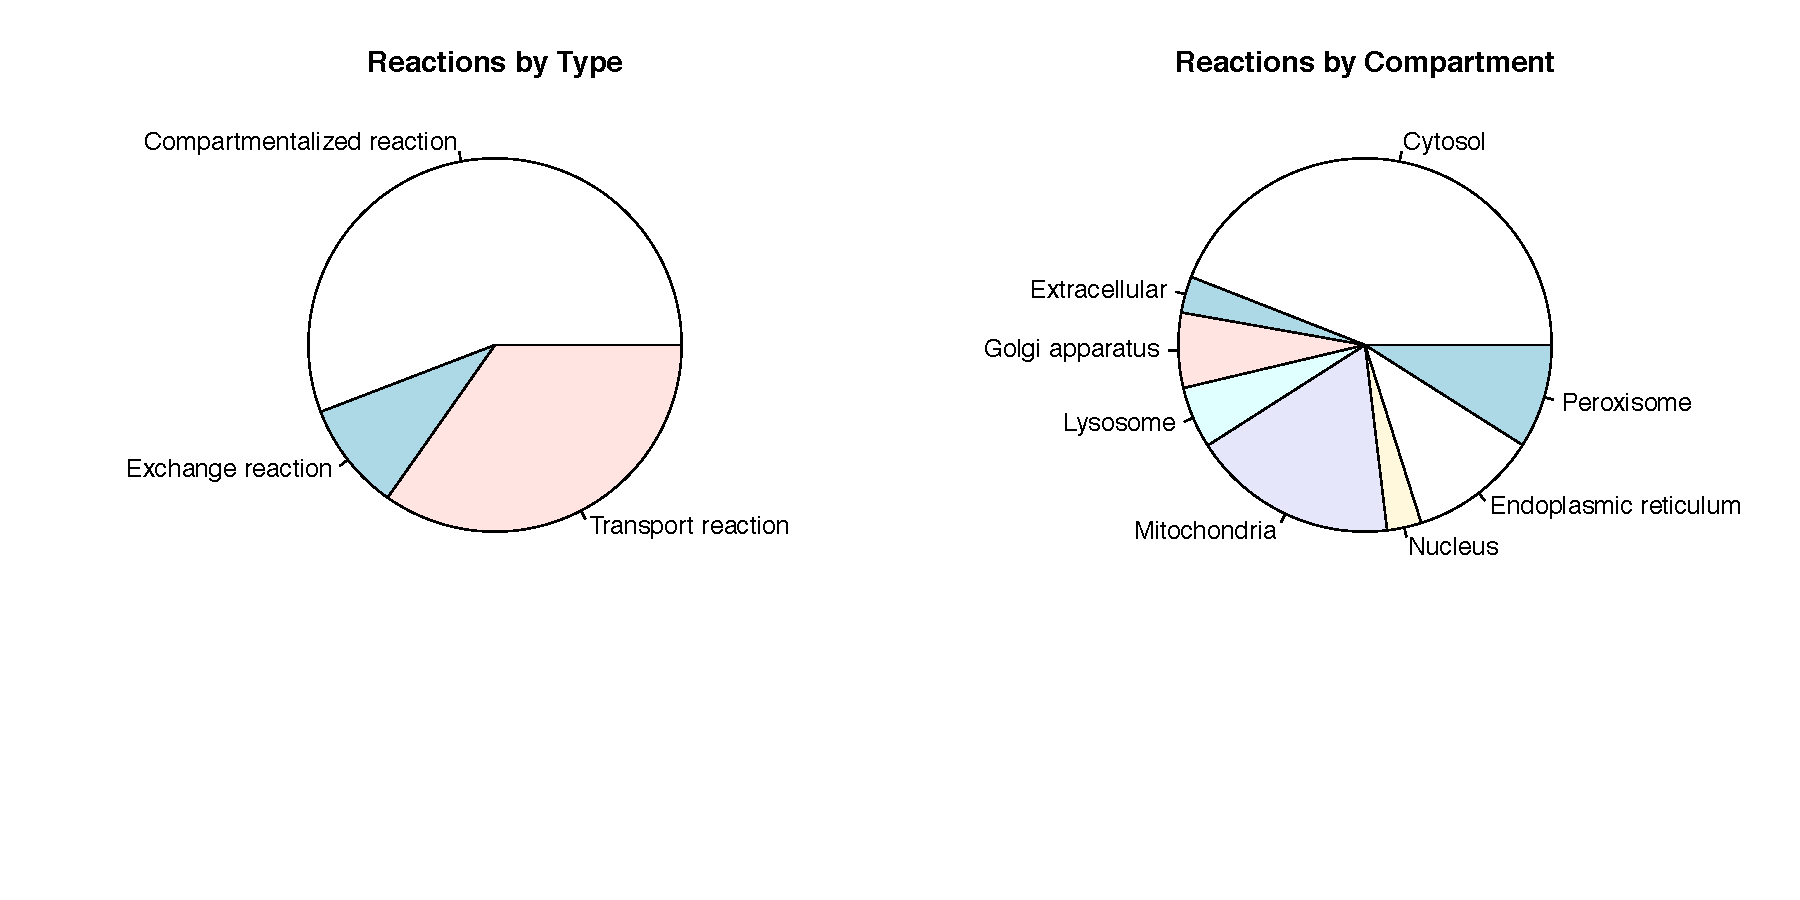
\includegraphics[width=\textwidth]{Fig1-Osorio-Gonzalez-Pinzon}
\caption{Distribution by type (left) and by compartments (right) of the reactions included into the RECON 2.04 Human Metabolic Reconstruction \citep{RECON2}.}
\end{figure}
\subsection{Stoichiometric matrix}
A metabolic reconstruction is often represented in a more compact form called the stoichiometry matrix (\textit{S}). If a metabolic reconstruction has \textit{n} reactions and \textit{m} participating metabolites, then the stoichiometry matrix will have correspondingly \textit{m} rows and \textit{n} columns. Values in the stoichiometric matrix represent the metabolite coefficients in each reaction. To generate the stoichiometric matrix of a metabolic reconstruction just type:
\begin{Schunk}
\begin{Sinput}
> stoichiometricMatrix(reactionList = glycolysisModel$REACTION)
\end{Sinput}
\begin{Soutput}
                                     reactions
metabolites                           R01 R02 R03 R04 R05 R06 R07 R08 R09 R10
  2-Phospho-D-glycerate[c]             -1   0   0   0   0  -1   0   0   0   0
  Phosphoenolpyruvate[c]                1   0   0   0   0   0   0   0   0  -1
  H2O[c]                                1   0   0   0   0   0   0   0   0   0
  D-Glyceraldehyde 3-phosphate[c]       0  -1  -1   1   0   0   0   0   0   0
  Glycerone phosphate[c]                0   1   0   1   0   0   0   0   0   0
  Orthophosphate[c]                     0   0  -1   0   0   0   0   0   0   0
  NAD+[c]                               0   0  -1   0   0   0   0   0   0   0
  3-Phospho-D-glyceroyl phosphate[c]    0   0   1   0   1   0   0   0   0   0
  NADH[c]                               0   0   1   0   0   0   0   0   0   0
  H+[c]                                 0   0   1   0   0   0   0   0   0   0
  beta-D-Fructose 1,6-bisphosphate[c]   0   0   0  -1   0   0   0   0   1   0
  ATP[c]                                0   0   0   0  -1   0  -1   0  -1   1
  3-Phospho-D-glycerate[c]              0   0   0   0  -1   1   0   0   0   0
  ADP[c]                                0   0   0   0   1   0   1   0   1  -1
  alpha-D-Glucose[c]                    0   0   0   0   0   0  -1   0   0   0
  alpha-D-Glucose 6-phosphate[c]        0   0   0   0   0   0   1  -1   0   0
  beta-D-Fructose 6-phosphate[c]        0   0   0   0   0   0   0   1  -1   0
  Pyruvate[c]                           0   0   0   0   0   0   0   0   0   1
                                     reactions
metabolites                           R11 R12 R13 R14 R15 R16 R17 R18 R19
  2-Phospho-D-glycerate[c]              0   0   0   0   0   0   0   0   0
  Phosphoenolpyruvate[c]                0   0   0   0   0   0   0   0   0
  H2O[c]                               -1   0   0   0   0   0   0   0   0
  D-Glyceraldehyde 3-phosphate[c]       0   0   0   0   0   0   0   0   0
  Glycerone phosphate[c]                0   0   0   0   0   0   0   0   0
  Orthophosphate[c]                     0   0   0  -1   0   0   0   0   0
  NAD+[c]                               0  -1   0   0   0   0   0   0   0
  3-Phospho-D-glyceroyl phosphate[c]    0   0   0   0   0   0   0   0   0
  NADH[c]                               0   0  -1   0   0   0   0   0   0
  H+[c]                                 0   0   0   0  -1   0   0   0   0
  beta-D-Fructose 1,6-bisphosphate[c]   0   0   0   0   0   0   0   0   0
  ATP[c]                                0   0   0   0   0  -1   0   0   0
  3-Phospho-D-glycerate[c]              0   0   0   0   0   0   0   0   0
  ADP[c]                                0   0   0   0   0   0   0   0  -1
  alpha-D-Glucose[c]                    0   0   0   0   0   0  -1   0   0
  alpha-D-Glucose 6-phosphate[c]        0   0   0   0   0   0   0   0   0
  beta-D-Fructose 6-phosphate[c]        0   0   0   0   0   0   0   0   0
  Pyruvate[c]                           0   0   0   0   0   0   0  -1   0
\end{Soutput}
\end{Schunk}
\subsection{Reactants and Products}
As described before, stoichiometric reactions represent the transformation of reactants into products in a chemical reaction. The \code{reactants} and \code{products} functions extract and return all reactants or products respectively in a stoichiometric reaction as a vector. If reaction is irreversible (\code{'=>'}) then reactants and products are separated and returned afterward as follows:
\begin{Schunk}
\begin{Sinput}
> reactants(reactionList = "ADP[c] + Phosphoenolpyruvate[c] => ATP[c] + Pyruvate[c]")
\end{Sinput}
\begin{Soutput}
[1] "ADP[c]"                 "Phosphoenolpyruvate[c]"
\end{Soutput}
\begin{Sinput}
> products(reactionList = "ADP[c] + Phosphoenolpyruvate[c] => ATP[c] + Pyruvate[c]")
\end{Sinput}
\begin{Soutput}
[1] "ATP[c]"      "Pyruvate[c]"
\end{Soutput}
\end{Schunk}
In reversible cases (\code{'<=>'})  all reactants at some point can act as products and \textit{vice versa}, for that reason both functions return all reaction metabolites:
\begin{Schunk}
\begin{Sinput}
> reactants(reactionList = "H2O[c] + Urea-1-Carboxylate[c] <=> 2 CO2[c] + 2 NH3[c]")
\end{Sinput}
\begin{Soutput}
[1] "H2O[c]"                "Urea-1-Carboxylate[c]" "CO2[c]"               
[4] "NH3[c]"               
\end{Soutput}
\begin{Sinput}
> products(reactionList = "H2O[c] + Urea-1-Carboxylate[c] <=> 2 CO2[c] + 2 NH3[c]")
\end{Sinput}
\begin{Soutput}
[1] "H2O[c]"                "Urea-1-Carboxylate[c]" "CO2[c]"               
[4] "NH3[c]"               
\end{Soutput}
\end{Schunk}

\subsection{Metabolites}
The \code{metabolites} function automatically identifies and lists all metabolites (with or without compartments) for a specific or a set of stoichiometric reactions.  This list is usually required for programs that perform FBA analysis as an independent input spreadsheet. In this example we show how to extract all metabolites (reactants and products) included in a metabolic reconstruction with and without compartments.
\begin{Schunk}
\begin{Sinput}
> metabolites(reactionList = glycolysisModel$REACTION)
\end{Sinput}
\begin{Soutput}
 [1] "2-Phospho-D-glycerate[c]"            "Phosphoenolpyruvate[c]"             
 [3] "H2O[c]"                              "D-Glyceraldehyde 3-phosphate[c]"    
 [5] "Glycerone phosphate[c]"              "Orthophosphate[c]"                  
 [7] "NAD+[c]"                             "3-Phospho-D-glyceroyl phosphate[c]" 
 [9] "NADH[c]"                             "H+[c]"                              
[11] "beta-D-Fructose 1,6-bisphosphate[c]" "ATP[c]"                             
[13] "3-Phospho-D-glycerate[c]"            "ADP[c]"                             
[15] "alpha-D-Glucose[c]"                  "alpha-D-Glucose 6-phosphate[c]"     
[17] "beta-D-Fructose 6-phosphate[c]"      "Pyruvate[c]"                        
\end{Soutput}
\begin{Sinput}
> metabolites(reactionList = glycolysisModel$REACTION, woCompartment = TRUE)
\end{Sinput}
\begin{Soutput}
 [1] "2-Phospho-D-glycerate"            "Phosphoenolpyruvate"             
 [3] "H2O"                              "D-Glyceraldehyde 3-phosphate"    
 [5] "Glycerone phosphate"              "Orthophosphate"                  
 [7] "NAD+"                             "3-Phospho-D-glyceroyl phosphate" 
 [9] "NADH"                             "H+"                              
[11] "beta-D-Fructose 1,6-bisphosphate" "ATP"                             
[13] "3-Phospho-D-glycerate"            "ADP"                             
[15] "alpha-D-Glucose"                  "alpha-D-Glucose 6-phosphate"     
[17] "beta-D-Fructose 6-phosphate"      "Pyruvate"                        
\end{Soutput}
\end{Schunk}
\subsection{Orphan Metabolites}
Those compounds that are not produced or consumed in any other reaction are generally called orphan metabolites, they represent one of the main causes of mass unbalances in metabolic reconstructions generating dead-ends without flux. The \code{orphanMetabolites} function extracts all orphan compounds included into a metabolic reconstruction.
\begin{Schunk}
\begin{Sinput}
> orphanMetabolites(reactionList = glycolysisModel$REACTION[noExchange])
\end{Sinput}
\begin{Soutput}
[1] "alpha-D-Glucose[c]" "Pyruvate[c]"        "H+[c]"             
[4] "H2O[c]"             "NAD+[c]"            "NADH[c]"           
[7] "Orthophosphate[c]" 
\end{Soutput}
\end{Schunk}
Due not all orphans are not consumed and not produced, the \code{orphanReactants} function, identifies compounds that are not produced internally by any other reaction and should be added to the reconstruction, for instance, as an input exchange reaction following the protocol proposed by \cite{Thiele2010}.
\begin{Schunk}
\begin{Sinput}
> orphanReactants(reactionList = glycolysisModel$REACTION[noExchange])
\end{Sinput}
\begin{Soutput}
[1] "alpha-D-Glucose[c]" "H+[c]"              "H2O[c]"            
[4] "NAD+[c]"            "NADH[c]"            "Orthophosphate[c]" 
\end{Soutput}
\end{Schunk}
By another side, the \code{orphanProducts} function, identifies compounds that are not consumed internally by any other reaction and should be added to the reconstruction, for instance, as an output exchange (sink) reaction.
\begin{Schunk}
\begin{Sinput}
> orphanProducts(reactionList = glycolysisModel$REACTION[noExchange])
\end{Sinput}
\begin{Soutput}
[1] "Pyruvate[c]"       "H+[c]"             "H2O[c]"           
[4] "NAD+[c]"           "NADH[c]"           "Orthophosphate[c]"
\end{Soutput}
\end{Schunk}
\subsection{Compartments}
As well as in eukaryotic cells, in which not all reactions occur in all compartments,  stoichiometric reactions in a metabolic reconstruction can be labeled to be restricted to a single compartment during FBA, by the assignment of a compartment label after each metabolite name. Some FBA implementations require the reporting of all compartments included in the metabolic reconstruction as an independent section of the human-readable input file. In this example, we show how to extract all compartments for all reactions included in the RECON 2.04 Human Metabolic Reconstruction \citep{RECON2}.
\begin{Schunk}
\begin{Sinput}
> compartments(reactionList = RECON$REACTION)
\end{Sinput}
\begin{Soutput}
[1] "c" "l" "m" "r" "e" "x" "n" "g"
\end{Soutput}
\end{Schunk}

\subsection{TSV files}
Additional to the SBML format, the TSV format is the default input of metabolic models for the \CRANpkg{sybil} R package. The TSV format is composed of three text files, following a character-separated (tab by default) value format where each line contains one entry (stoichiometric reaction and associated info). The \code{writeTSVmod} function can write a metabolic model in a TSV format as follows:
\begin{Schunk}
\begin{Sinput}
> writeTSVmod(modelData = glycolysisModel,
+           modelID = "Glycolysis",
+           outputFile = "glycolysis")
\end{Sinput}
\end{Schunk}
Metabolic models in TSV format can be readed through the \code{readTSVmod} function included in the \CRANpkg{sybil} package:
\begin{Schunk}
\begin{Sinput}
> sybil::readTSVmod(prefix = "glycolysis",quoteChar = "\"")
\end{Sinput}
\begin{Soutput}
model name:             Glycolysis 
number of compartments  1 
                        [c] 
number of reactions:    19 
number of metabolites:  18 
number of unique genes: 22 
objective function:     +1 R00200 
\end{Soutput}
\end{Schunk}
\section{Summary}
We introduced the \pkg{minval} package to check the syntax validity, evaluate the mass-charge balance and extract all orphan metabolites of a set of stoichiometric reactions. Together, this steps represent the minimal validation that should be performed in a genome-scale metabolic reconstruction. Functions to characterize and export metabolic models in SBML and TSV formats as well as to extract all reactants, products, metabolite names and compartments for a set of stoichiometric reactions were also introduced. Moreover, we also show in a step by step fashion, how this minimal evaluation process of mass balance can avoid an overestimation of the the net yield of pyruvate from an alpha-D-glucose molecule when using an unbalanced model of the glycolysis pathway.

\section{Acknowledgements}
DO and JG  were supported by the Pontificia Universidad Javeriana (Grant ID 5619, 6235, 6371, 6375). We thank to the anonymous reviewers for their helpful comments and suggestions to improve the package.
\bibliography{Osorio-Gonzalez-Pinzon.bib}

\address{Daniel Osorio\\
Grupo de Investigación en Bioinformática y Biología de Sistemas\\
Instituto de Genética, Universidad Nacional de Colombia\\
Bogotá\\
Colombia\\}
\email{dcosorioh@unal.edu.co}

\address{Janneth Gonzalez\\
Grupo de Investigación en Bioquímica Experimental y Computacional\\
Facultad de Ciencias, Pontificia Universidad Javeriana\\
Bogotá\\
Colombia\\}
\email{janneth.gonzalez@javeriana.edu.co}

\address{Andres Pinzon\\
Grupo de Investigación en Bioinformática y Biología de Sistemas\\
Instituto de Genética, Universidad Nacional de Colombia\\
Bogotá\\
Colombia\\}
\email{ampinzonv@unal.edu.co}
